For X10-udtag er der udviklet en række diagrammer ud fra applikationsmodel metoden.
På figur \ref{fig:X10_udtag_domain} er domænemodellen som resten af diagrammerne er udviklet ud fra.
Der er et sekvensdiagram på figur \ref{fig:X10_udtag_SD} for alle de aktuelle use-cases som beskriver systemets virkemåde.
Ud fra dette er der lavet et klassediagram på figur \ref{fig:X10_udtag_Class} som dækker de forskellige use-cases med controller klasser og kommunikationen til CSS hovedenheden via X10.


\begin{figure}[!htb] \centering
\centering 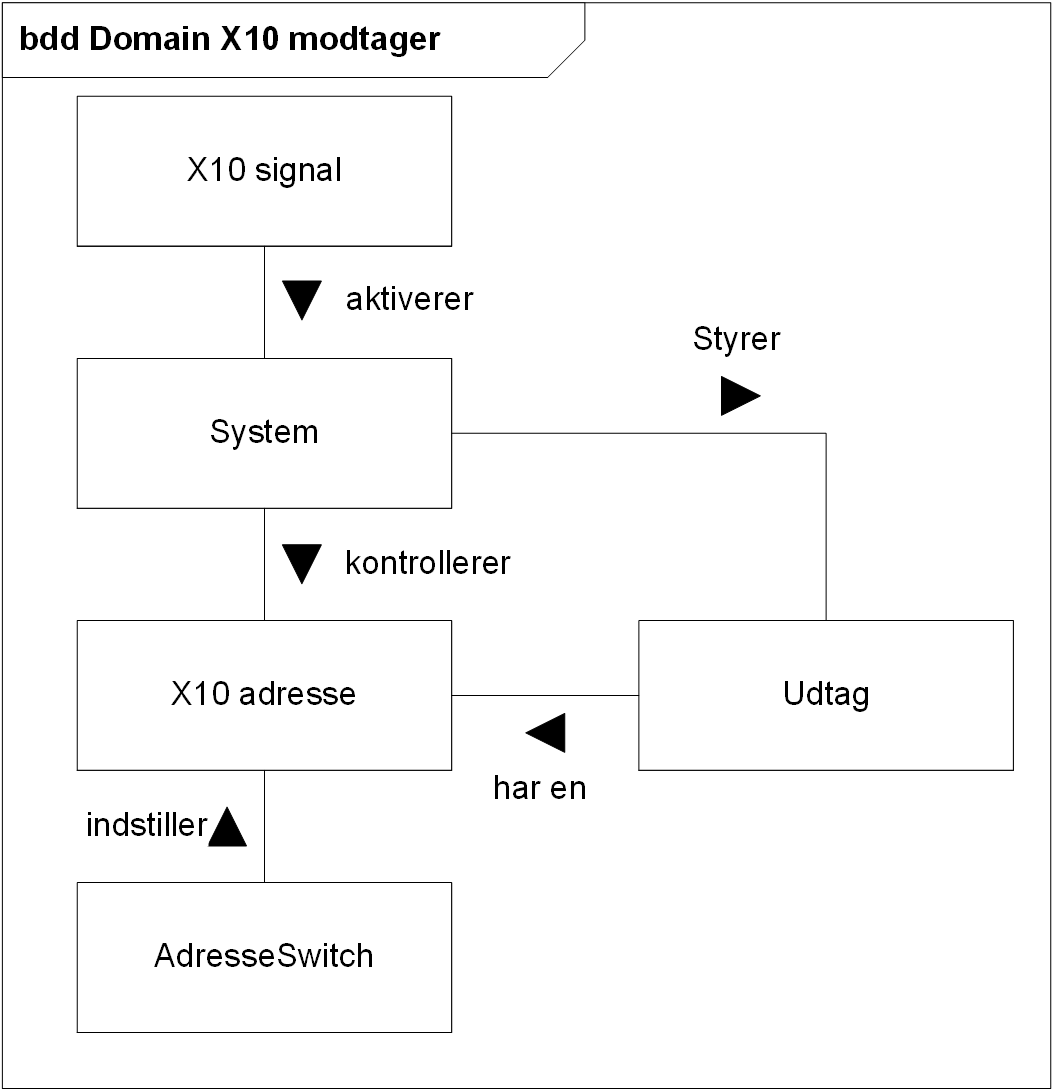
\includegraphics[width=0.6\textwidth]{billeder/uml/X10_modtager_Domain}
     \caption{Domænemodel for X10-udtag}
     \label{fig:X10_udtag_domain}
\end{figure}

\begin{figure}[!htb]
	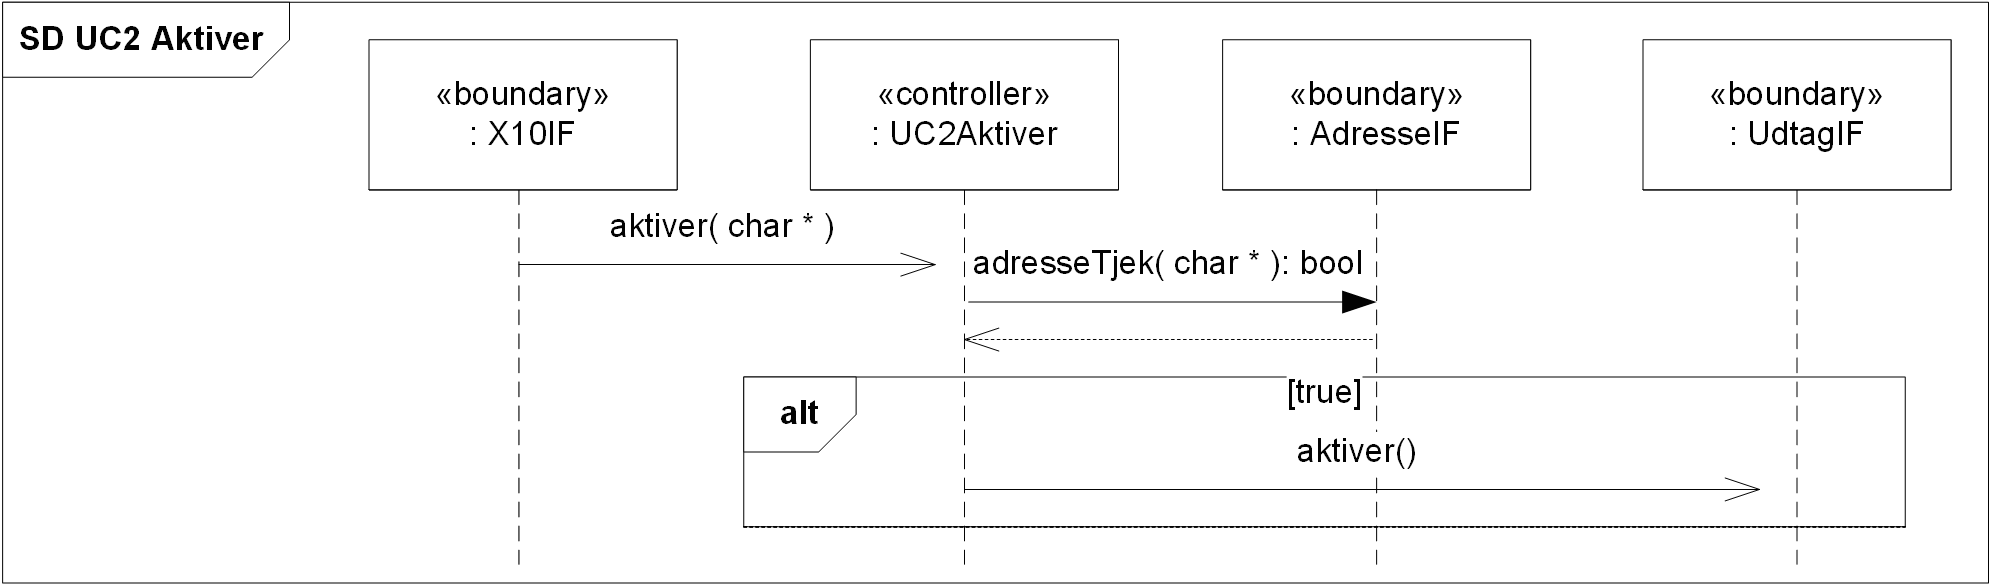
\includegraphics[width=\textwidth]{billeder/uml/X10_modtager_SD}
     \caption{Use-case sekvensdiagrammer for X10-udtag}
     \label{fig:X10_udtag_SD}
\end{figure}

\begin{figure}[!htb]
     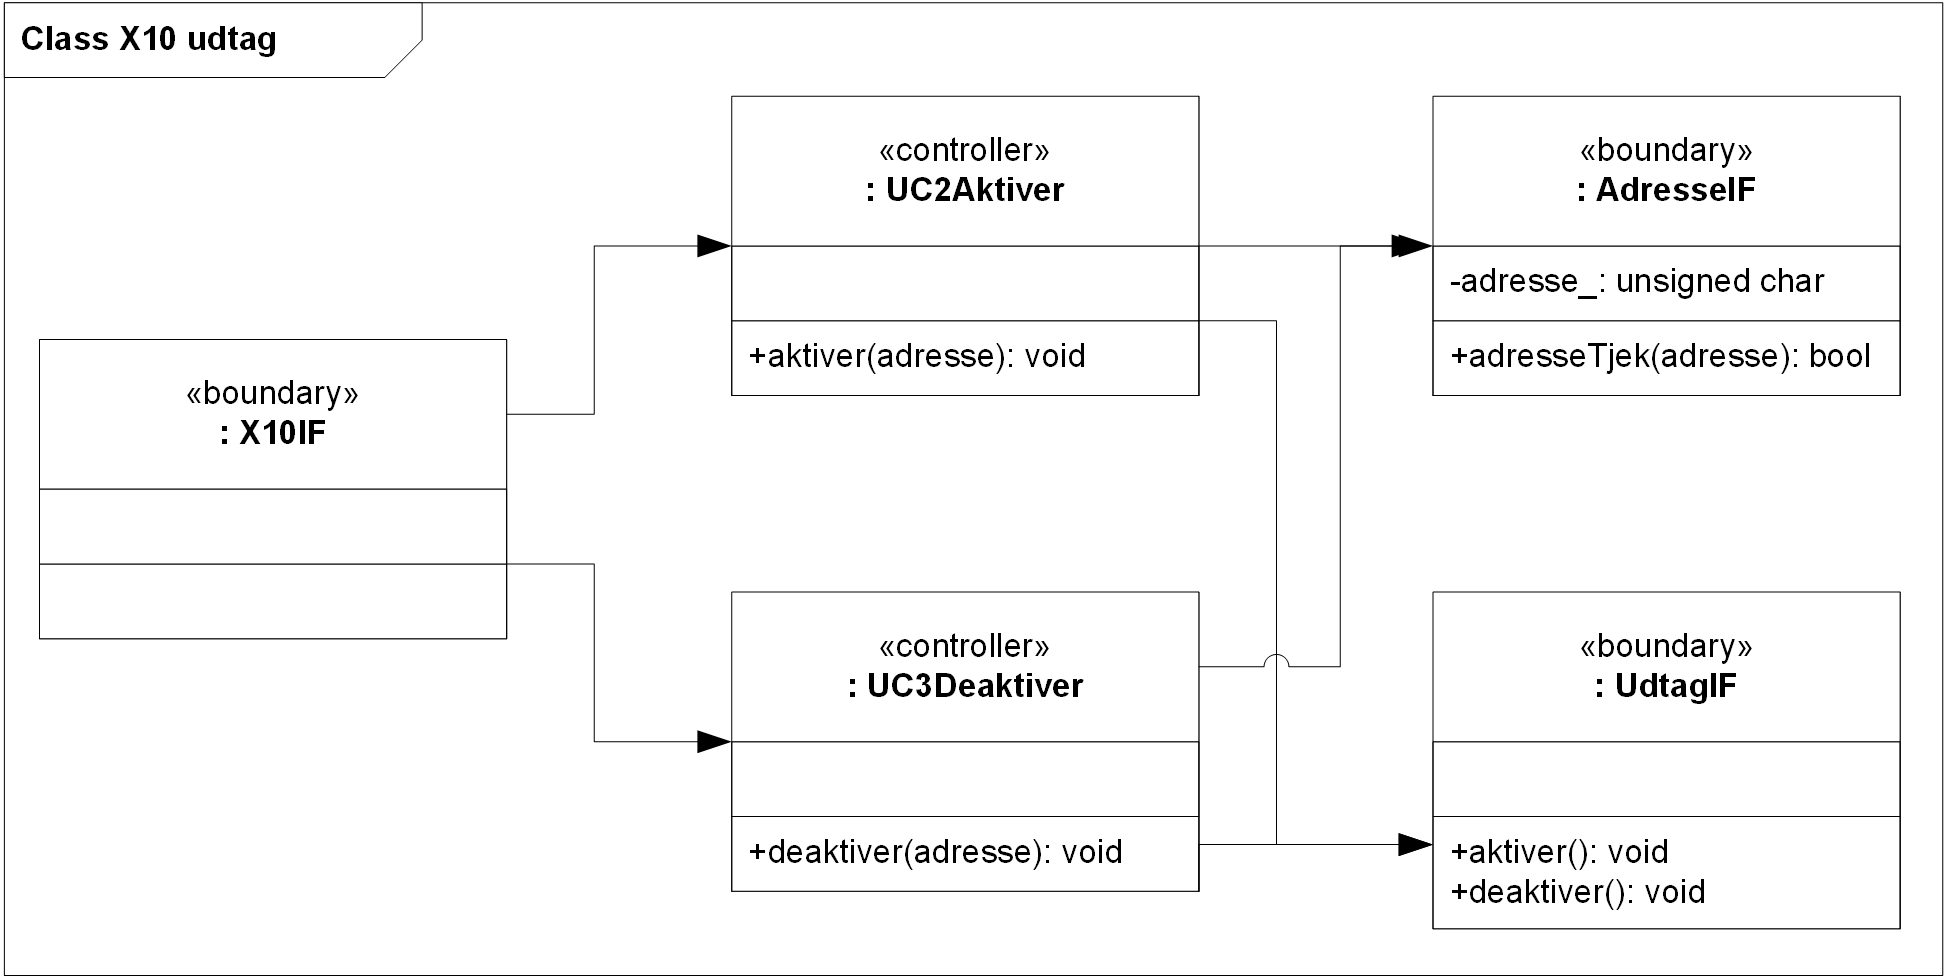
\includegraphics[width=\textwidth]{billeder/uml/X10_modtager_Class}
     \caption{Klassediagram for X10-udtag}
     \label{fig:X10_udtag_Class}
\end{figure}


For at få et endeligt funktionsdygtigt system, er der i designfasen og implementeringen lavet en række støtte metoder til klasserne og en global funktion. Den globale funktion er lavet for at kunne bruge X10IF klassens interupt funktioner, som understøtter hardware signaler udefra, under microcontrollerens interupt service rutine. Det endelige klassediagram ses på figur \ref{fig:X10_udtag_Class_Staric}. 


\begin{figure}[!htb]
     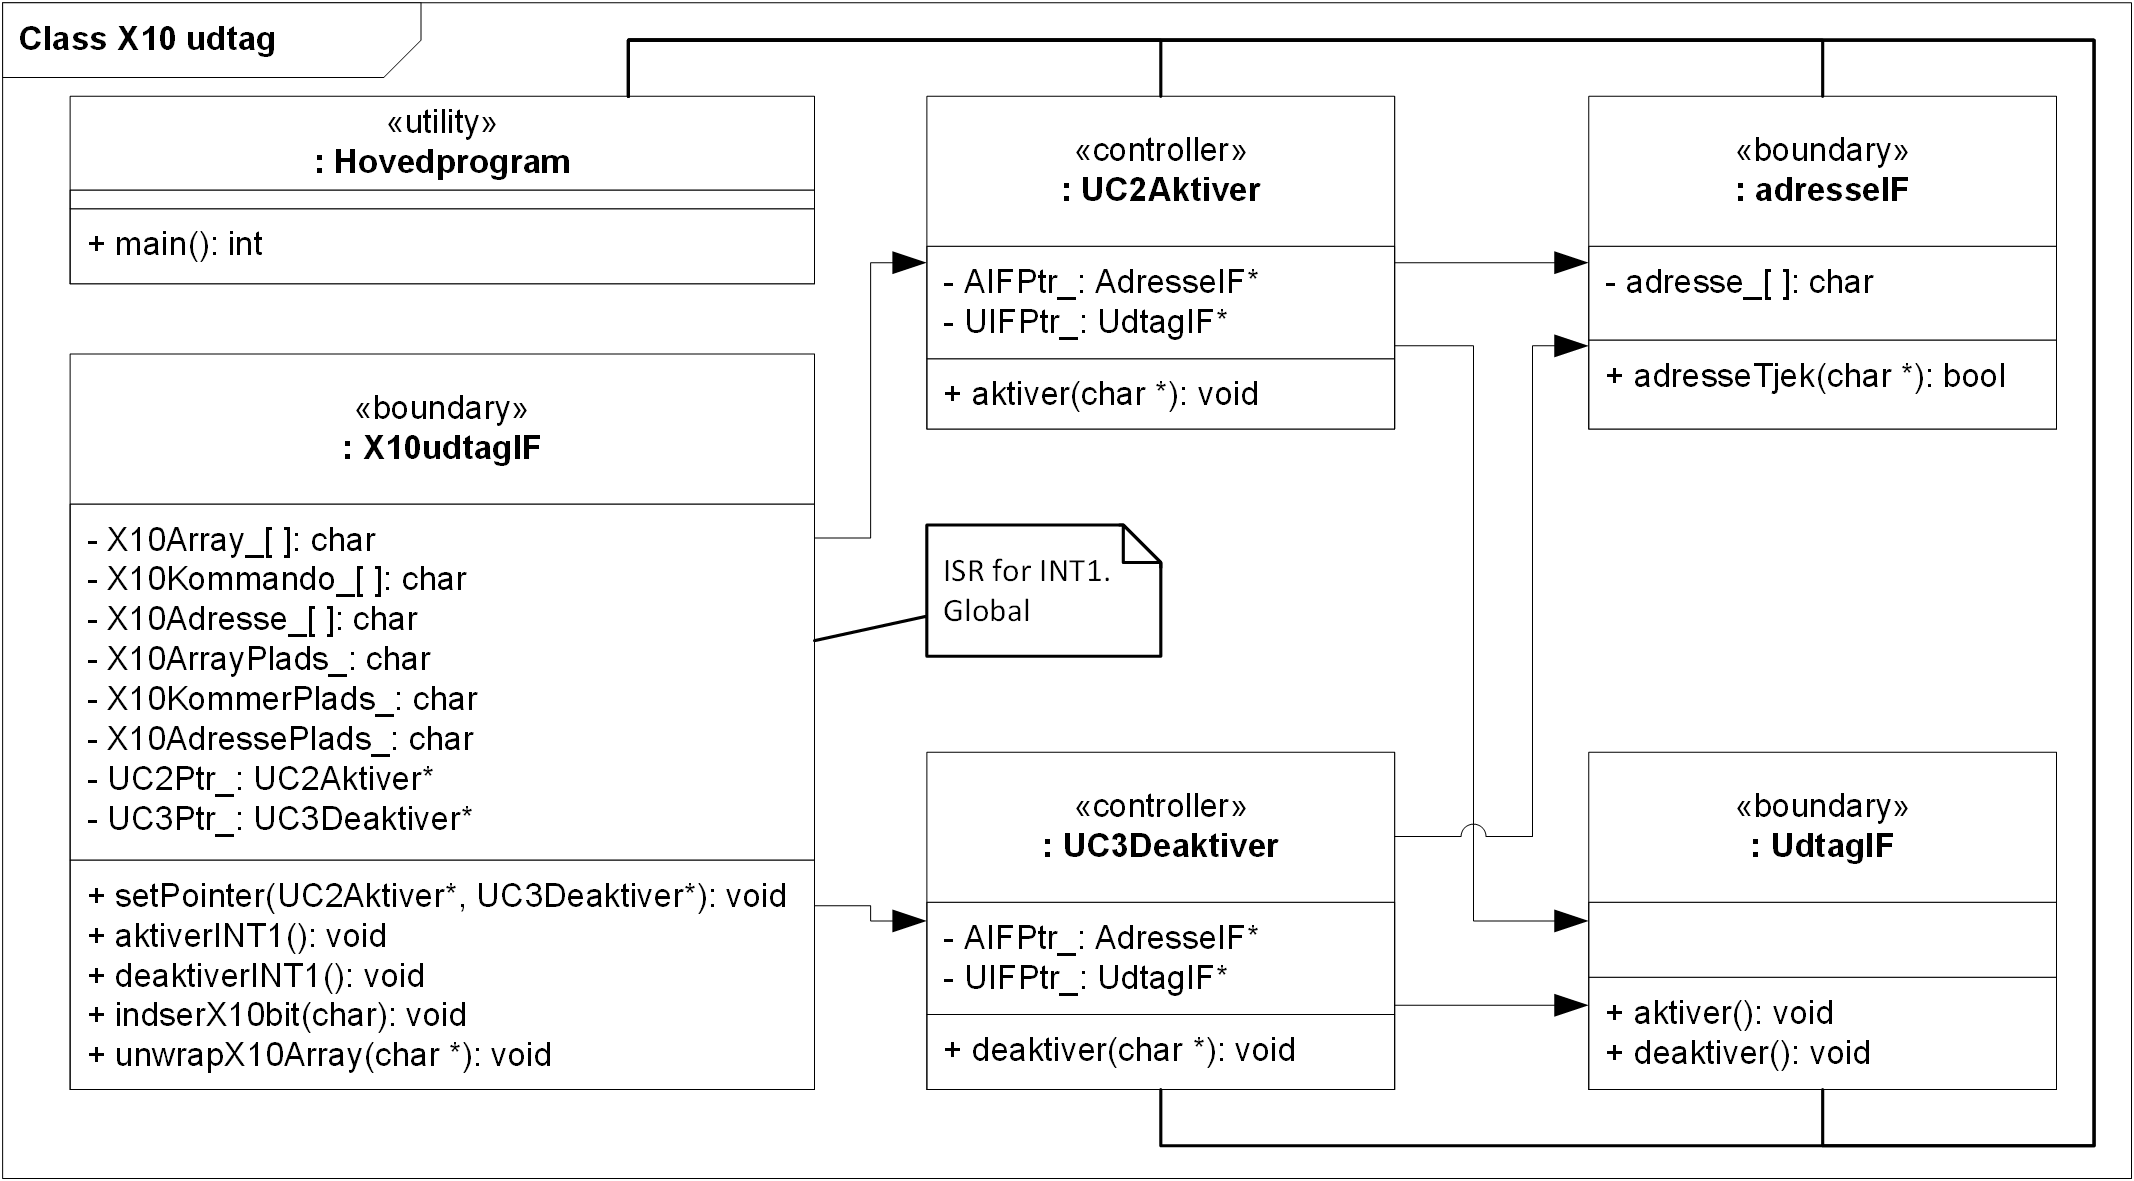
\includegraphics[width=\textwidth]{billeder/uml/X10_modtager_Class_Static}
     \caption{Statisk Klassediagram for X10-udtag}
     \label{fig:X10_udtag_Class_Staric}
\end{figure}